\documentclass[main]{subriles}

\begin{document}
    \subsection{Сферическое отображение и основной оператор}

    \begin{definition}
        $\Phi$ --- поверхность, гладкая, регулярная, $f: D \ra \R^3$,$\Phi = f(D)$
        \[\Gamma: \Phi \ra \cancel{\R^3} S^2 \text{ --- отобр } x \mapsto \ol{n}(x)\]
        Такое отображение называется \ul{сферическим}
        %рисунок 10_1 плоскости с вектором вверх, рисунок сферы
        \begin{figure}[H]
            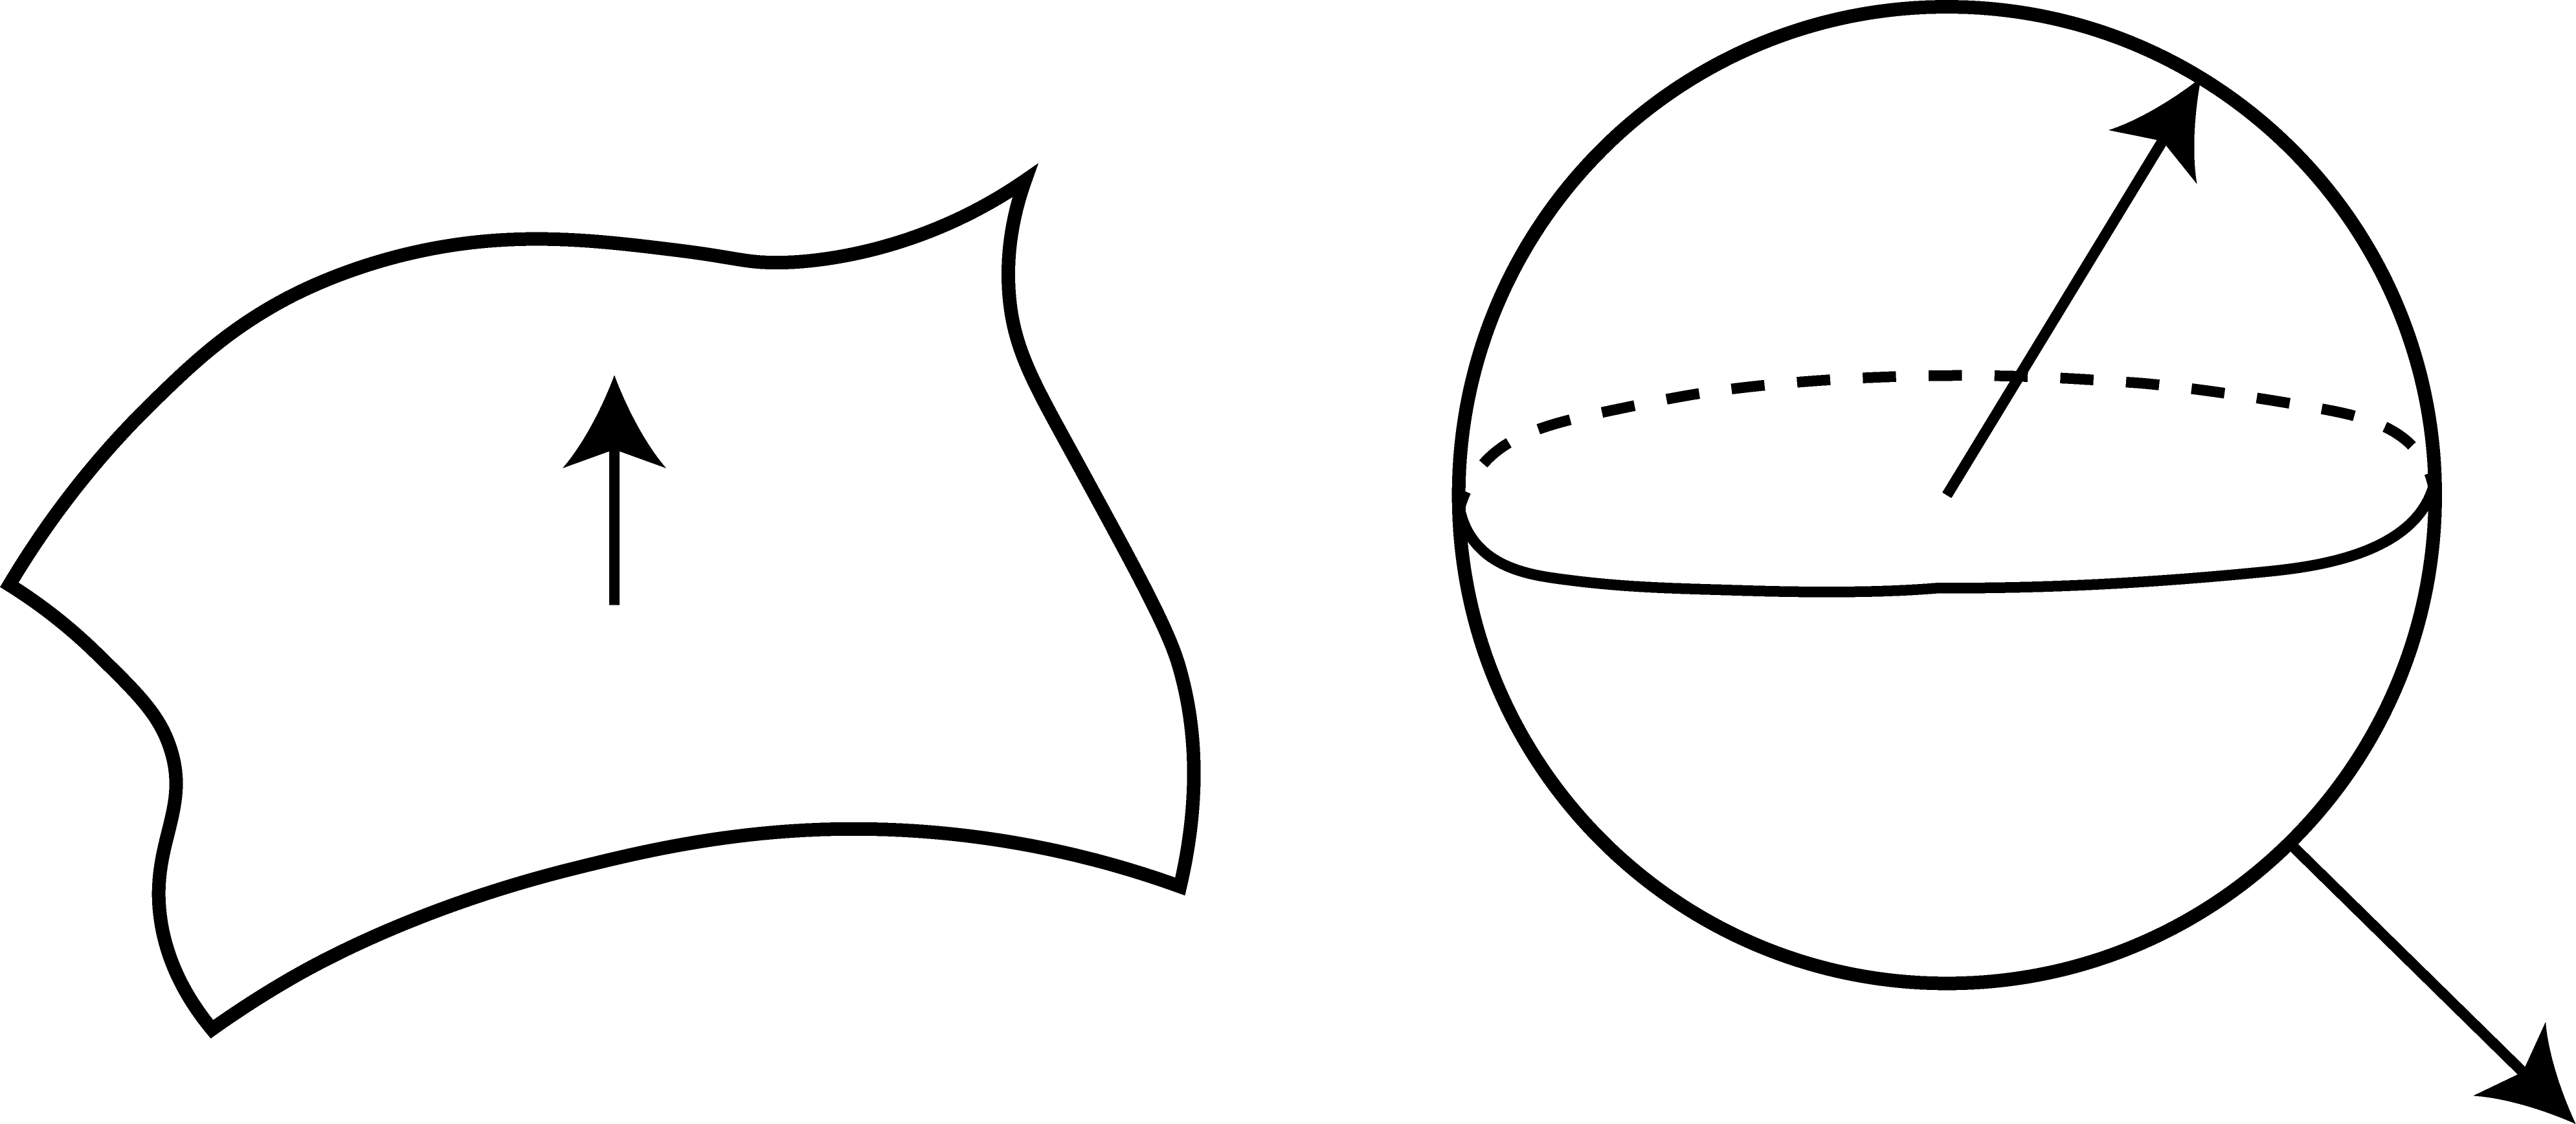
\includegraphics[width=7cm]{pics/10_1.png}
            \centering
        \end{figure}

    \end{definition}

    \begin{examples}
        \begin{enumerate}
          \item $\Phi$ --- сфера радиуса 1\\
          $\Gamma(x) = x$\\
          $\Phi$ --- сфера, радиуса R
          \[\Gamma(x) = \frac{x}{|x|}\]
          \item $\Phi$ --- плоск., $\Gamma(x)=\const$
          %рисунок 10_2 плоскости
            \begin{figure}[H]
                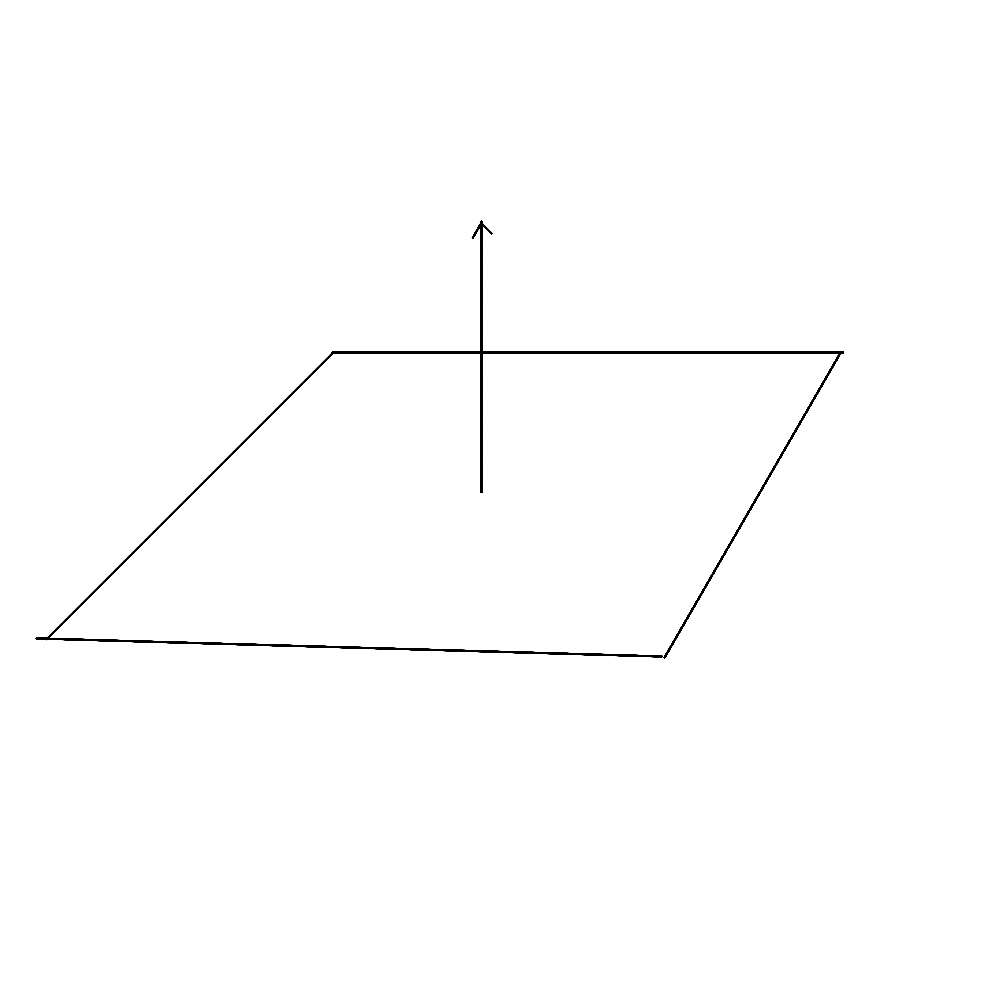
\includegraphics[width=3.5cm]{pics/10_2.png}
                \centering
            \end{figure}

        \end{enumerate}
    \end{examples}

    \begin{definition}
        \ul{Основной оператор} пов-ти --- дифференциал данного отображения $\Gamma$\\ \ \\
        Т.е. это линейный оператор $x \in \R$
        \[R_x: \R^2 \ra \R^2\]
        \[\forall \vec{w} \in \R^2\]
        \[x = f(u_0,\ v_0)\]
        \[R_x(\vec{w})=\lim_{\alpha \ra 0} \frac{\Gamma(f(u_0;\ v_0) + \alpha \vec{w}) - \Gamma(f(u_0;\ v_0))}{\alpha} \text{ --- вектор в кас. плоскости $S^2$}\]
        (в числителе единичные векторы, точнее их производные)\\
        %рисунок 10_1 поверхности с D и отображения
        \begin{figure}[H]
            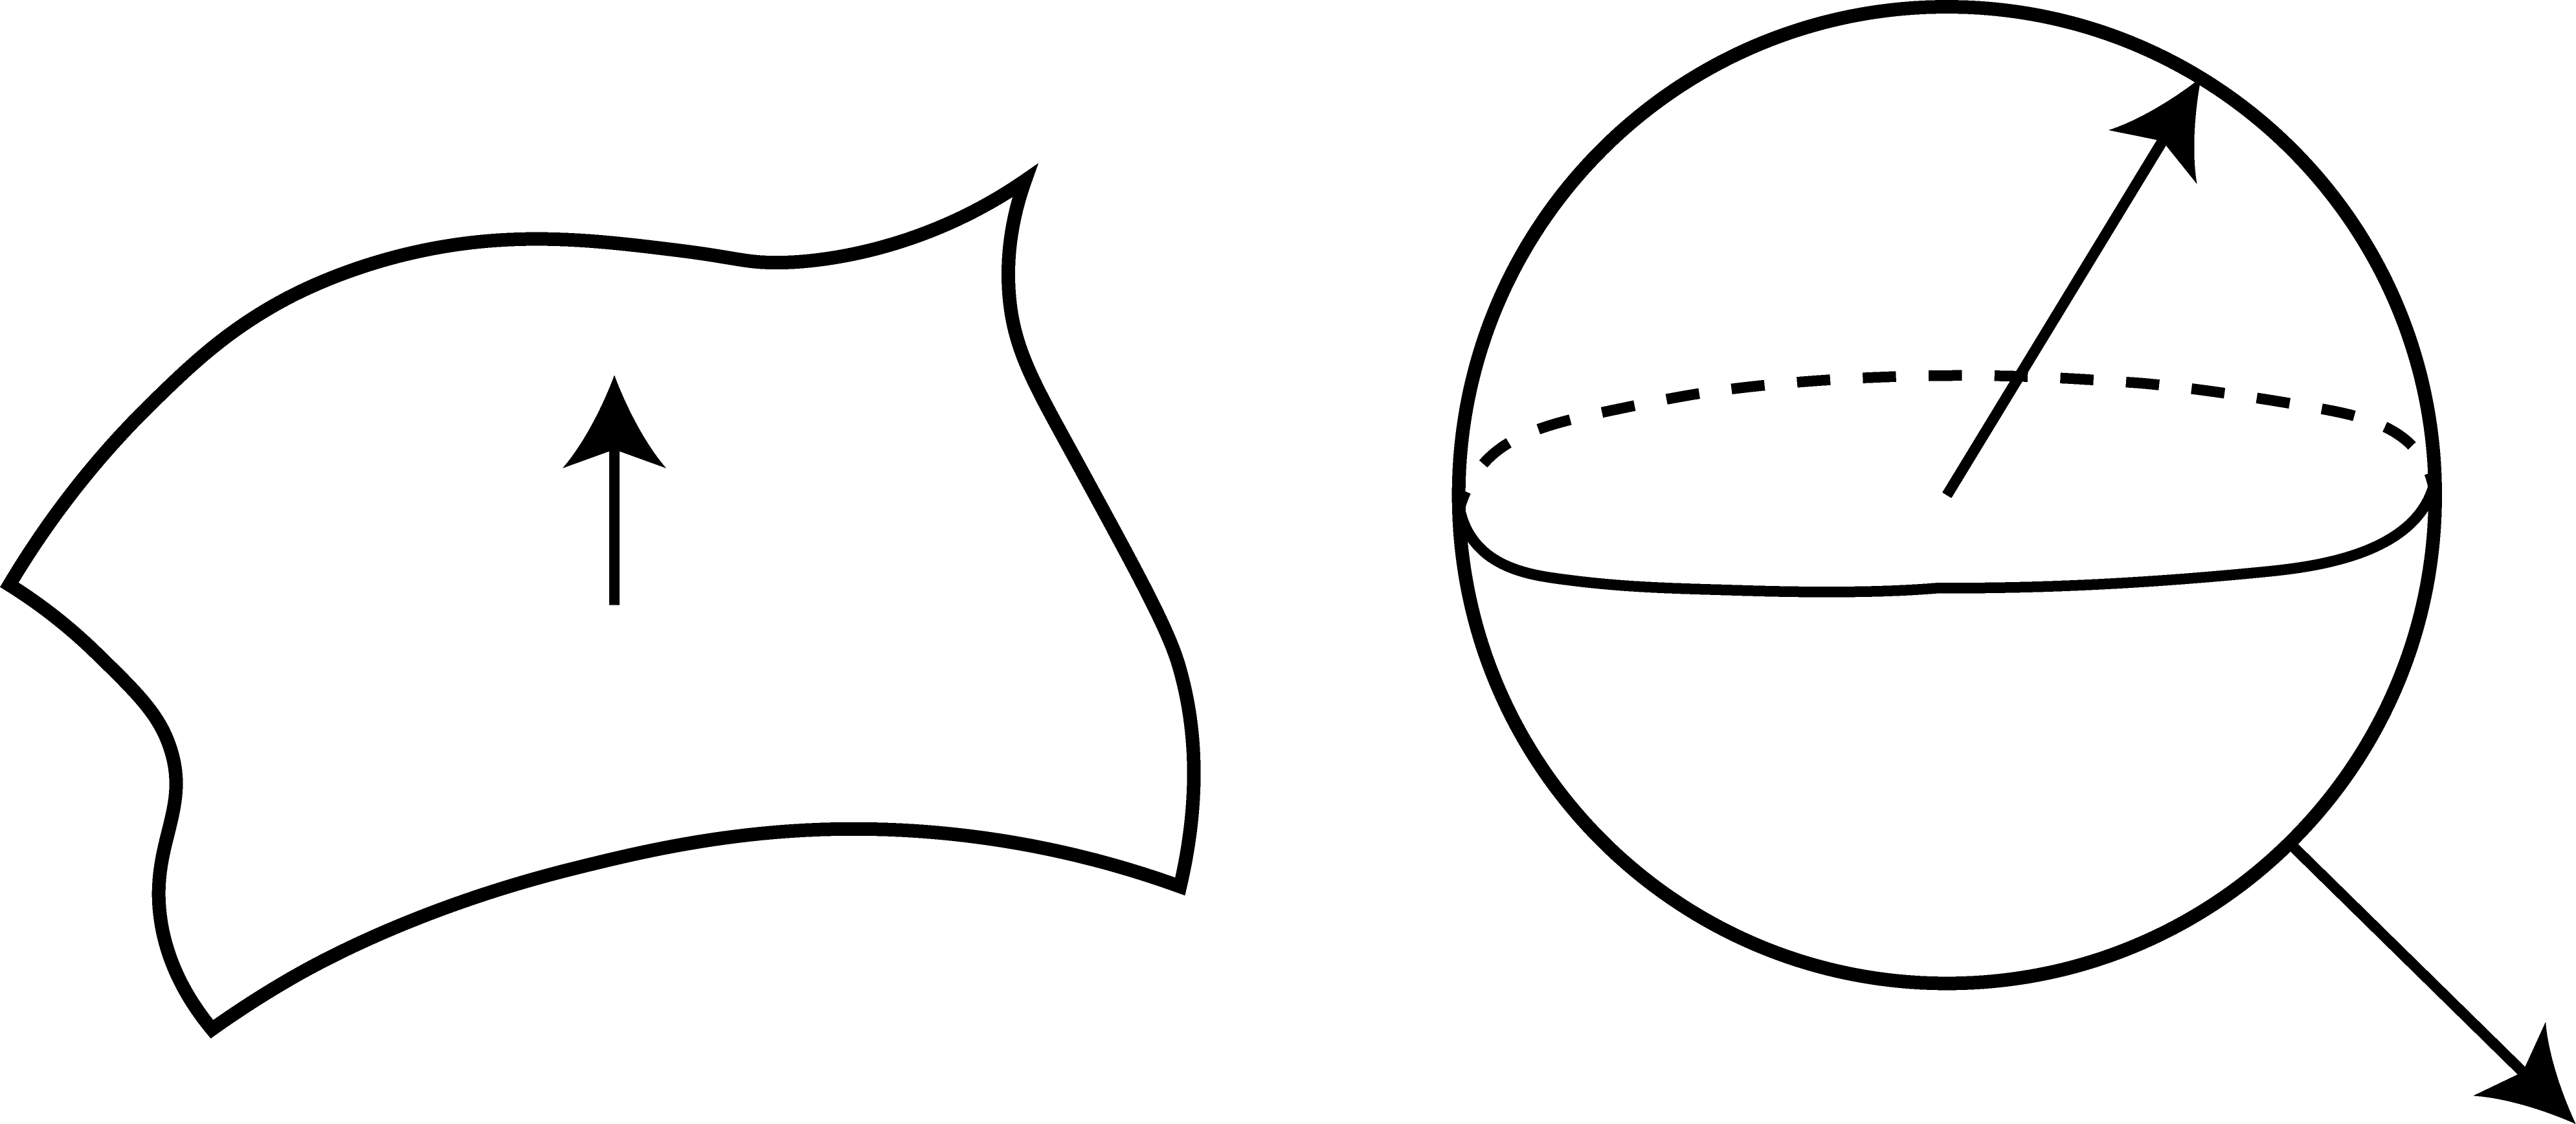
\includegraphics[width=7cm]{pics/10_1}
            \centering
        \end{figure}

    \end{definition}

    \begin{Example}\
        %рисунок 10_3 с отображением \Gamma
        \begin{figure}[H]
            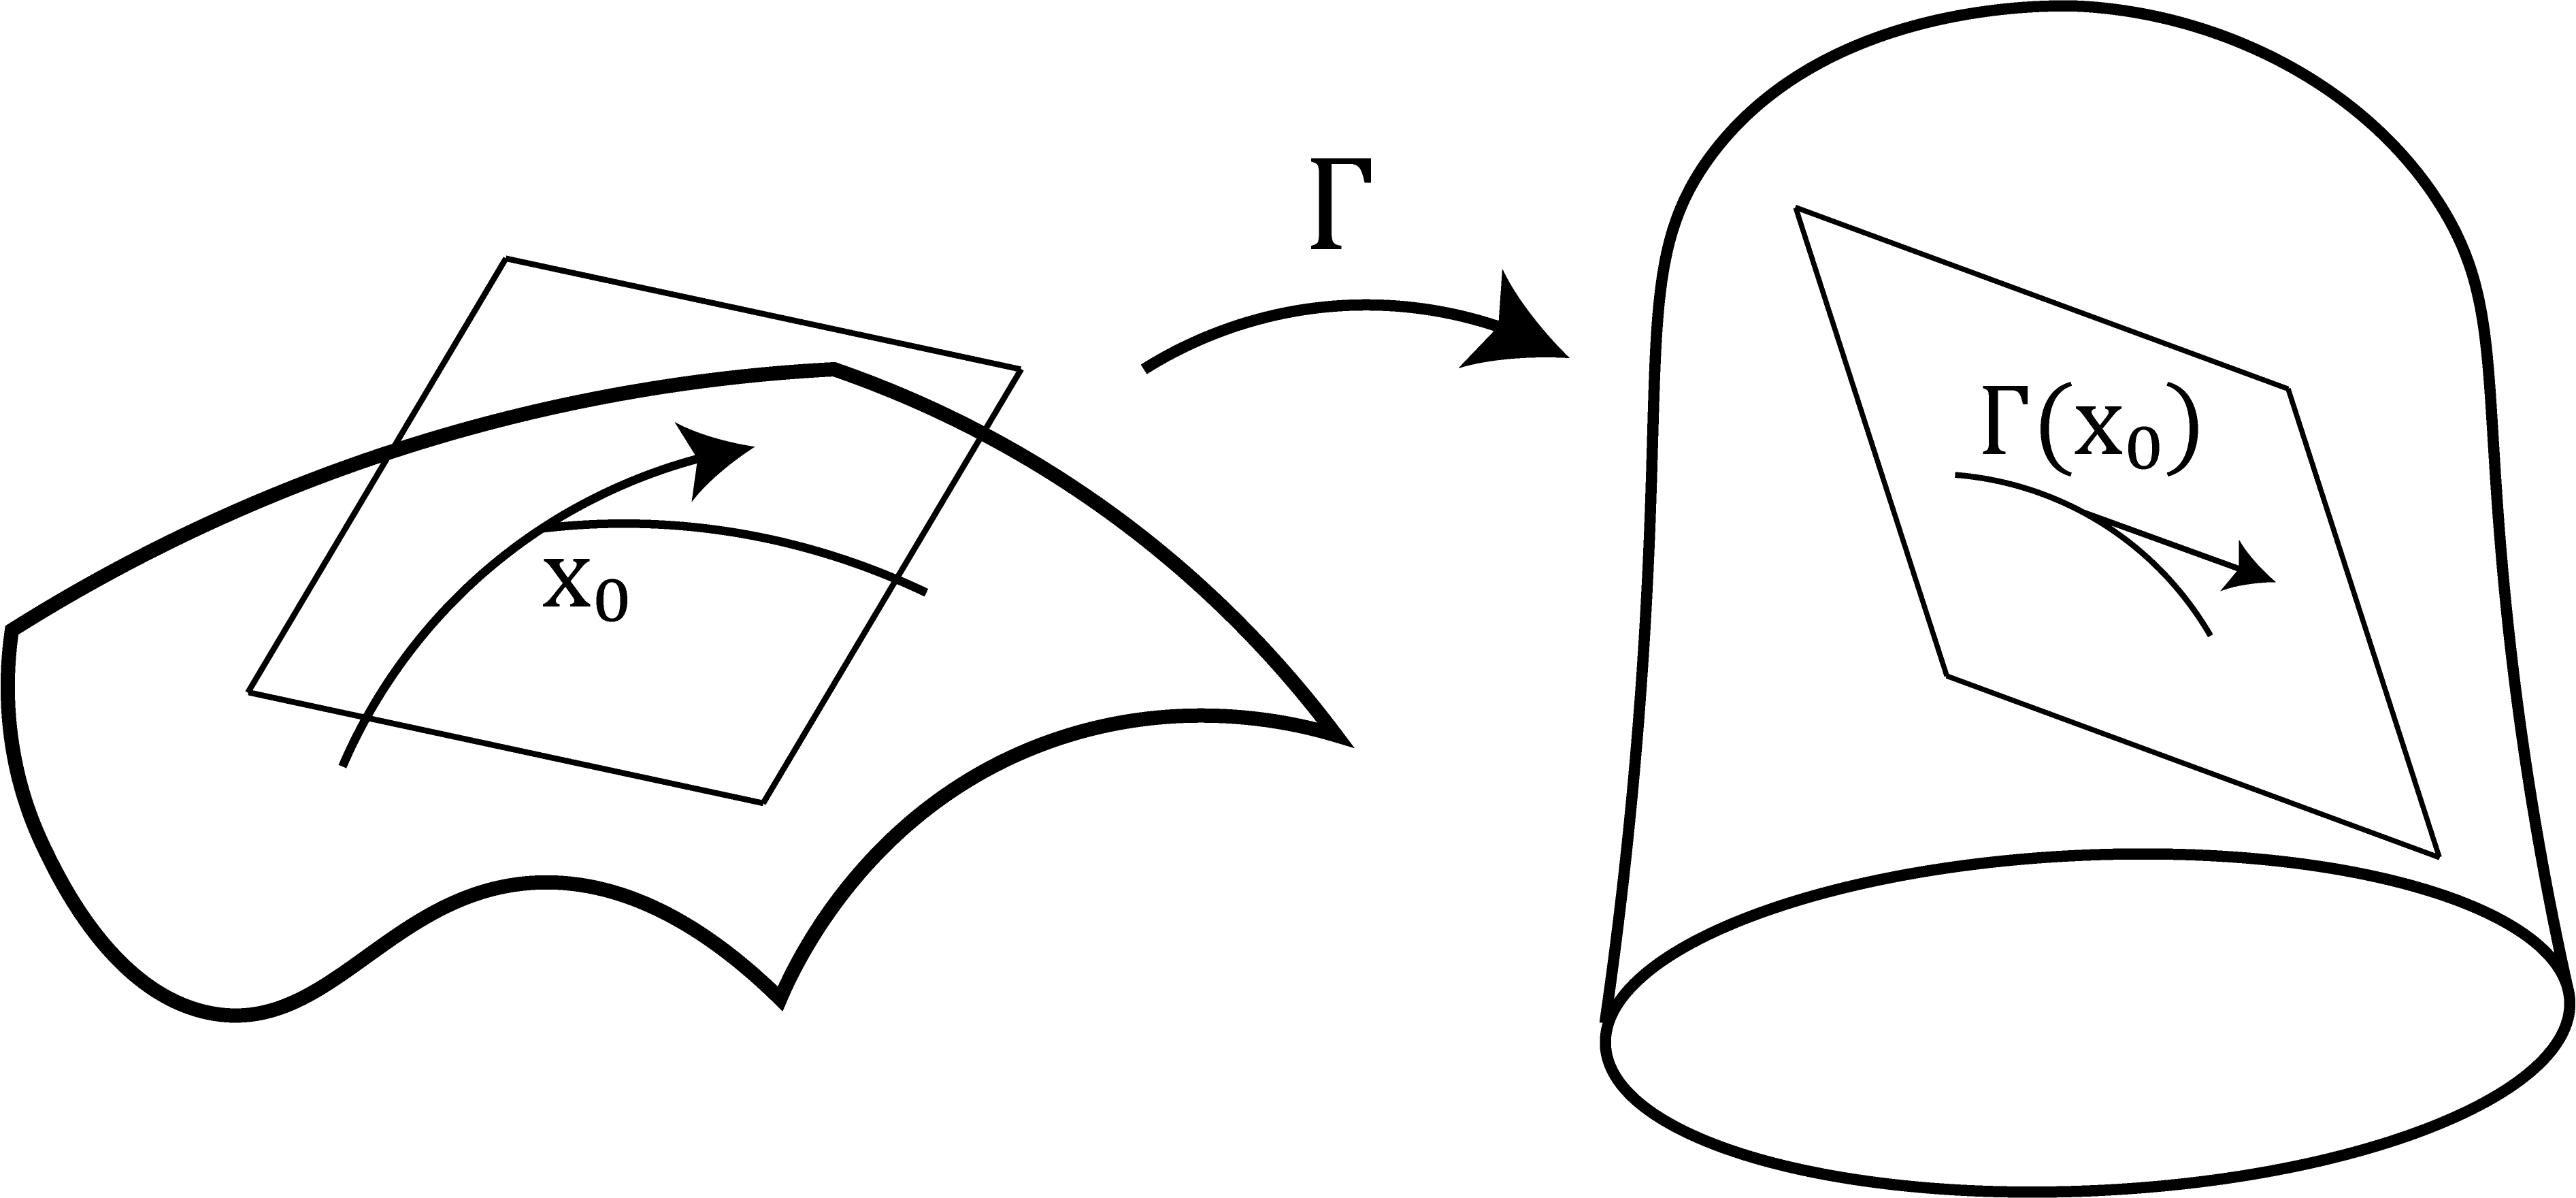
\includegraphics[width=8cm]{pics/10_3.png}
            \centering
        \end{figure}

    \end{Example}

    Сама функция $R_x(\vec{w})$ работает как производная, это некоторый вектор. Его можно разложить по базису

    Пусть $w_1 = u,\q w_2 = v$, тогда
    \[\frac{R_x(w_1)}{|R_x(w_1)|}0,\ \frac{R_x(w_2)}{|R_x(w_2)|}\text{ --- базисные векторы}\]

    \subsection{Теорема Родрига}
    \begin{theorem}[Родриг]
        С.ч. основного оператора --- главные кривизны со знаками минус ($-k_1$ и $-k_2$), а с.в. --- главные направления
    \end{theorem}

    \begin{theorem}
        Пусть координатные линии поверхности совп. с главными направлениями
        \[\RA n_u = - k_1 f_u \qq n_v = - k_2 f_v,\]
        где $f_u,\ f_v$ --- производные по $u$ и по $v$
    \end{theorem}

    \begin{Remark}[теоремы равносильны]
        \[\begin{matrix}
            n_u = R_x(1,\ 0)\\
            n_v = R_x(0,\ 1)
        \end{matrix} \q \begin{matrix}
            f_u = (1,\ 0)\\
            f_v = (0,\ 1)
        \end{matrix} \text{ в кас. плоск. пов.}\]
        Потому что у пов. есть два с.ч.
    \end{Remark}

    Как мы выбирали систему координат?
    \[\begin{cases}
        x = u\\
        y = v\\
        z = \varphi(u,\ v)\\
        \text{н. коорд. }(0,0,0)\\
        \varphi(0,0) = 0
    \end{cases}\]
    Также мы выбирали, чтобы кас. пл-ть $z=0$\\
    %рисунок 10_4 кас. плосктости с $z=0$
    \begin{figure}[H]
        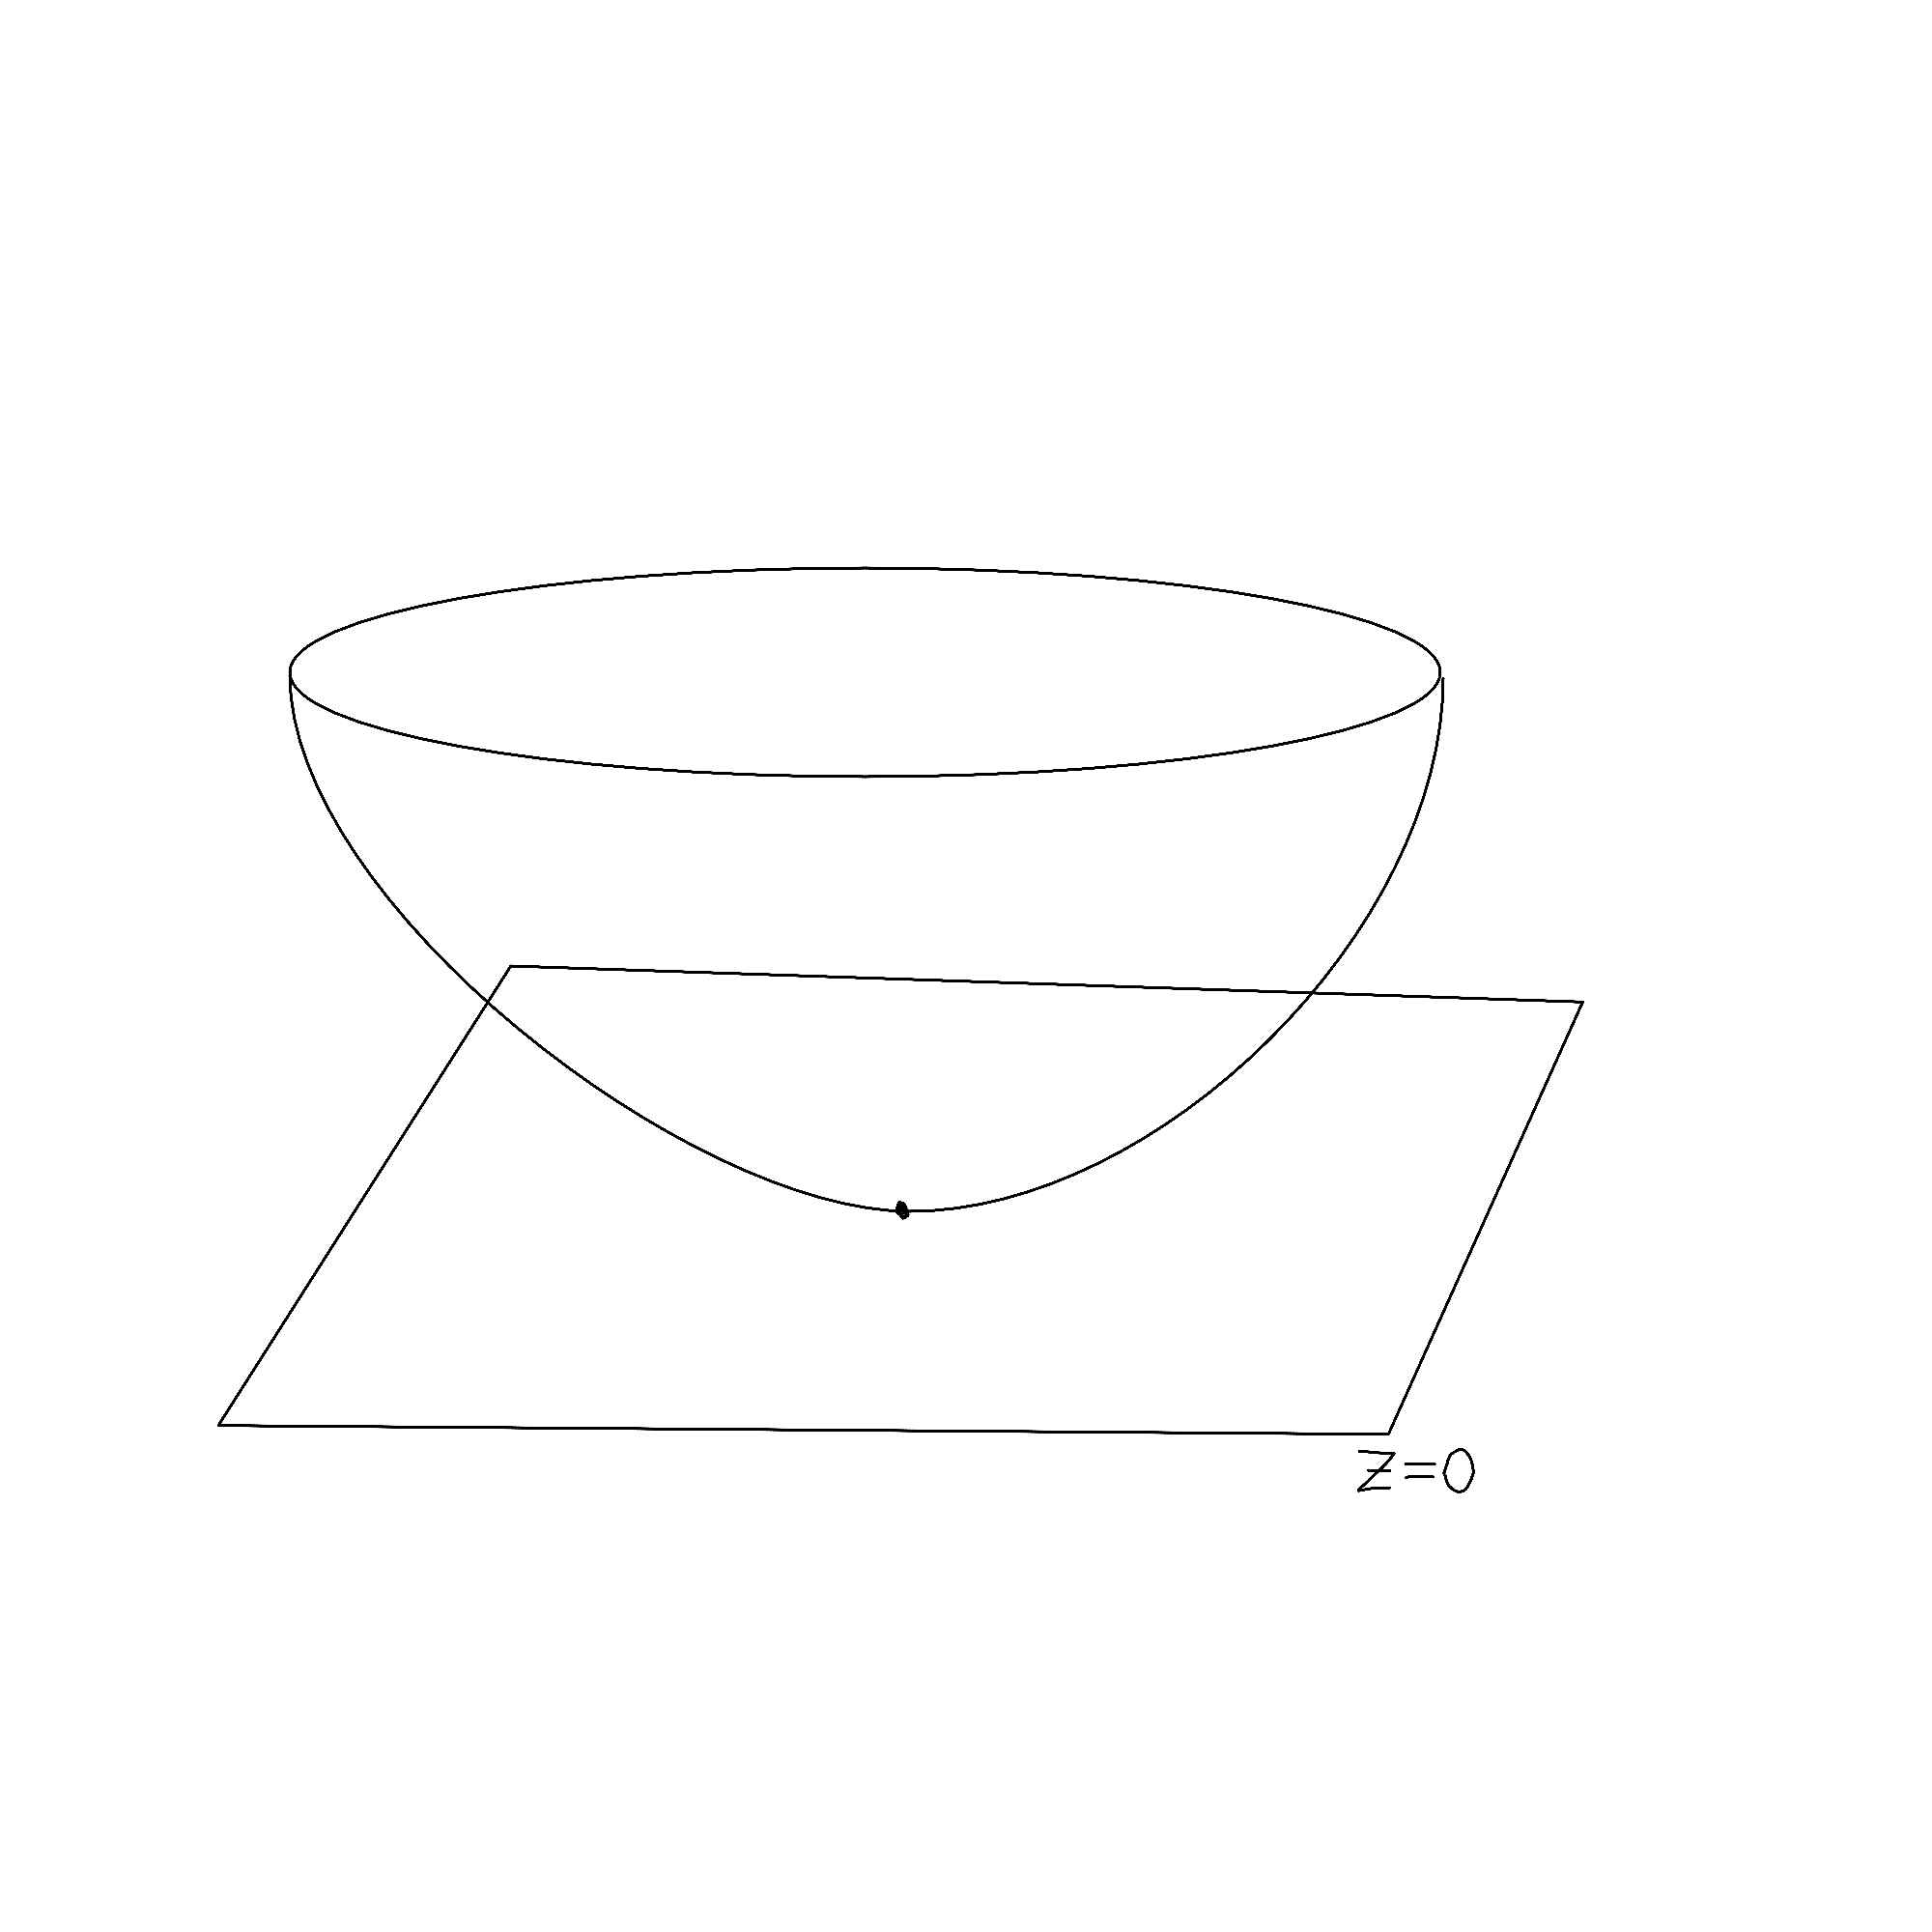
\includegraphics[width=4cm]{pics/10_4.png}
        \centering
    \end{figure}

    т.е. $\varphi_u(0,0) = 0 \q \varphi_v(0,0) = 0 $\\
    Что мы делали?
    \[\varphi_{uu}(0,0) = L,\q \varphi_{uv}(0,0) = M,\q \varphi_{vv}(0,0) = N\]
    \[z = Lx^2 + 2 Mxy + Ny^2\]
    Что мы вспоминали? Можем выбрать так парабалоид, чтобы при $x,y$ координаты равнялись 0, то есть координатные длины совпали с главными направлениями
    т.е. $M = 0 = \varphi_{uv}(0,0)$\\ \ \\
    Давайте что-нибудь посчитаем
    \[f(u,v) = (u,v, \varphi(u,v))\]
    \[f_u = (1,\ 0,\ \varphi_u)\]
    \[f_v = (0,\ 1,\ \varphi_v)\]
    \[\ol{n} = \frac{f_u \times f_v}{|f_u \times f_v|} = \frac{(-\varphi_u;\ -\varphi_v;\ 1)}{\sqrt{1 + \varphi_u^2 + \varphi_v^2}}\]
    \[n_u = \Br{- \frac{\varphi_u}{\sqrt{}},\
    - \frac{\varphi_v}{\sqrt{}},\
    \frac{1}{\sqrt{}}}_u = \]
    \[\Br{(\sqrt{1 + \varphi_u^2 + \varphi_v^2})_u =
    \frac{\varphi_u \varphi_{uu} + \varphi_v \varphi_{uv}}{\sqrt{1 + \varphi_u^2 + \varphi_v^2}}}\]
    \[= \Br{-\frac{\varphi_{uu}\sqrt{...} - \varphi_u \frac{\varphi_u \varphi_{uu} + \varphi_v \varphi_{vv}}{\sqrt{...}}}{1+ \varphi_u^2 + \varphi_v^2};
    - \frac{\varphi_{vu} \sqrt{...} - \varphi_v \frac{...}{...}}{1 + \varphi_u^2 + \varphi_v^2};
    -\frac{1}{(1+ \varphi_u^2 + \varphi_v^2)^{\frac{3}{2}}} (\varphi_u \varphi_{uv} + \varphi_v \varphi_{uv})}\]
    Наш корень в $(0,0,0)$ равняется 1, $\varphi_{uv}=0$ как мы договорились, аналогично остальные, используем это:
    \[n_u \Big|_{(0,0,0)} = \Br{-\varphi_{uu},\ 0,\ 0} = -k_1 \cdot (1,\ 0,\ 0)\]
    \[k_1 = \varphi_{uu} \qq f_u = (1,\ 0,\ \varphi_u)\]
    \[n_v \text{ - аналогично (первая 0, вторая не 0, ...)}\]
    \[n_v \Big|_{(0,0,0)} = (0,\ -\varphi_{vv},\ 0) = -k_2 (0,\ 1,\ 0) = -k_2 f_v\]

    \subsection{Связь гауссовой кривизны и сферического отображения}
    \begin{theorem}
        $\w{D}$ --- область на поверхности
        \[\lim_{diam(\w{D}) \ra 0}\frac{S(\Gamma(\w{D}))}{S(\w{D})} = |K|\]
        "Мера на сколько изменилась"{}
        %рисунок 10_5
        \begin{figure}[H]
            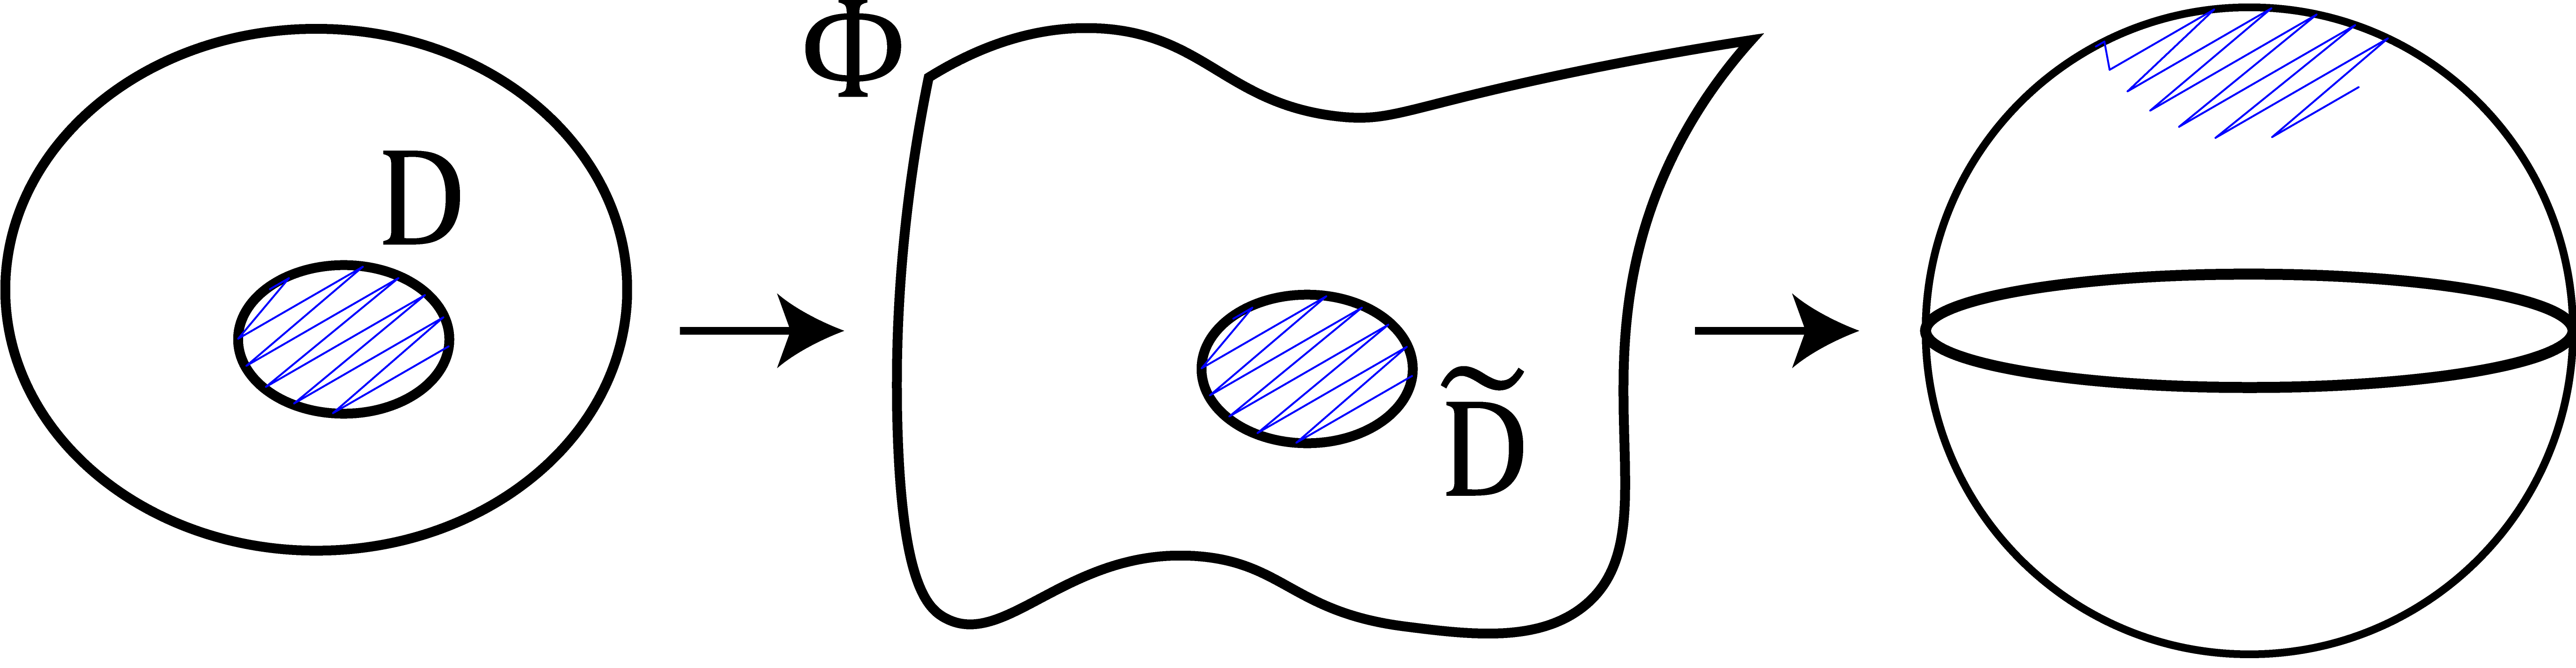
\includegraphics[width=9cm]{pics/10_5.png}
            \centering
        \end{figure}

    \end{theorem}

    \begin{Proof}
        \[S(\w{D}) = \iint_D |\ol{f}_u \times \ol{f}_v| du dv \us{\text{т. о среднем}}{=} S(D) |f_u \times f_v| \Big|_{(u_0,v_0)}\]
        \[S(\Gamma(\w{D})) = \iint_D |n_u \times n_v| du dv \us{\text{т. о среднем}}{=} |n_u \times n_v| \Big|_{(u_0, v_0)} S(D)\]
        \[\lim_{diam \w{D} \ra 0} \frac{S(\Gamma(\w{D}))}{S(\w{D})} = \lim \frac{|n_u \times n_v|\Big|_{u_0,v_0} \cancel{S(D)}}{|f_u \times f_v| \Big|_{(u_0,v_0)} \cancel{S(D)}} = \frac{|n_u \times n_v|}{|f_u \times f_v|}\]
        Введем специальные координаты, чтобы направления совпадали с главными ($u,v$ - главн.) (насколько это переход к частному случаю? Нужно понять, что $n_u \times n_v$ не зависит от выбора координат)

        Тогда у нас есть теорема Родрига:
        \[n_u = -k_1 f_u \qq n_v = -k_2 f_v\]
        \[\Ra \frac{|n_u \times n_v|}{|f_u \times f_v|} = |(-k_1)(-k_2)| = |K|\]
    \end{Proof}

    \subsection{Деривационные формулы. Вычисление $n_u \times n_v$}
    \begin{remark}
        Являются аналогами формул Френе.
    \end{remark}

    У нас есть три вектора: $(\ol{r}_u,\ \ol{r}_v,\ \ol{n})$ --- базис
    \[r_{uu} = \Gamma_{11}^1 r_u + \Gamma_{11}^2 r_v + \alpha \ol{n}\]
    \[r_{uv} = \Gamma_{12}^1 r_u + \Gamma_{12}^2 r_v + \beta \ol{n}\]
    \[r_{vv} = \Gamma_{22}^1 r_u + \Gamma_{22}^2 r_v + \gamma \ol{n}\]
    \[n_u = \alpha_1 r_u + \beta_1 r_v + \gamma_1 \ol{n}\]
    \[n_v = \alpha_2 r_u + \beta_2 r_v + \gamma_2 \ol{n}\]
    \[\Gamma_{ij}^k \text{ наз. символами Кристоффеля}\]
    \[\text{Факт. } \Gamma_{ij}^k \text{ относ. к внутр. геометрии (б/д)}\]
    Заметим, что $\alpha = L,\ \beta = M,\ \gamma = N$ --- коэф. \RNumb{2} формы
    \[L := r_{uu} \cdot n = \Gamma_{11}^1 \ub{=0}{r_u \cdot n} + \alpha \ub{=1}{\ol{n} \cdot \ol{n}} + \Gamma_{11}^2 \ub{=0}{f_v \cdot n}\]
    Заметим, что $\gamma_1 = \gamma_2 = 0$, т.к. $|\ol{n}| = 1 \Ra \ol{n}_u \bot \ol{n}$, значит:
    \[r_{uu} = \Gamma_{11}^1 r_u + \Gamma_{11}^2 r_v + L \ol{n}\]
    \[r_{uv} = \Gamma_{12}^1 r_u + \Gamma_{12}^2 r_v + M \ol{n}\]
    \[r_{vv} = \Gamma_{22}^1 r_u + \Gamma_{22}^2 r_v + N \ol{n}\]
    \[n_u = \alpha_1 r_u + \beta_1 r_v \ |\cdot r_u\]
    \[n_v = \alpha_2 r_u + \beta_2 r_v \]
    \[r_u n_u = \alpha_1 E + \beta_1 F\]
    \[r_v n_u = \alpha_1 F + \beta_1 G\]
    \[r_u n_v = \alpha_2 E + \beta_2 F\]
    \[r_v n_v = \alpha_2 F + \beta_2 G\]
    \[0 = (r_u \cdot n)_u = \ub{=L}{r_{uu} n} + r_u n_u \RA -L = r_u n_u\]
    \[0 = (r_v \cdot n)_u = \ub{=-M}{r_{uv}} + r_v n_u\]
    \[\text{Аналогично }-M = r_v n_u = r_u n_v \text{ и } -N = r_v n_v\]
    \[\alpha_1 = \frac{\begin{vmatrix}
      -L & F\\
      -M & G
    \end{vmatrix}}{\begin{vmatrix}
      E & F\\
      F & G
    \end{vmatrix}} = \frac{MF - LG}{EG - F^2} \text{ из системы сост. ур-ий (Крамер)}\]
    \[\beta_1 = \frac{LF - ME}{EG - F^2}\]
    \[\alpha_2 = \frac{NF - MG}{EG - F^2}\]
    \[\beta_2 = \frac{MF - NE}{EG - F^2}\]
\end{document}
